\begin{frame}{Automap: Next Steps}

\begin{itemize}[<+->]
\item demonstrate automap on more challenging problem(s)
\begin{itemize}
\item move beyond proof of concept\dots
\item try to show effects on evolvability \& solution quality
\item soft-bodied robots (?)
\end{itemize}
\item explore using generative adversarial networks (GANs) in place of autoencoders
\item put in conversation with learning theory \& evolvability synthesis \cite{kouvaris2017evolution}
\end{itemize}

\end{frame}


\begin{frame}{Challenges + Solutions}

\textbf{Manual G-P map design is difficult and highly heuristic\dots but deep
learning implementation is too!}
\pause
\vspace{-1ex}
\begin{itemize}[<+->]
\itemsep0em
\item learn better quality G-P maps than manually designed?
\end{itemize}
\vspace{-1ex}
\pause


\textbf{Computational cost of making training data.}
\pause
\vspace{-1ex}
\begin{itemize}[<+->]
\itemsep0em
\item parallelism
\end{itemize}
\vspace{-1ex}
\pause


\textbf{Autoencoder performance limitations}
\pause
\vspace{-1ex}
\begin{itemize}[<+->]
\itemsep0em
\item ANN autoencoders: active area of research
\item G-P autoencoder map could use other ``back end''
\end{itemize}

\end{frame}

\begin{frame}{Toy Result: Evolvability Signature}

\begin{figure}
  \begin{subfigure}[b]{0.33\linewidth}
    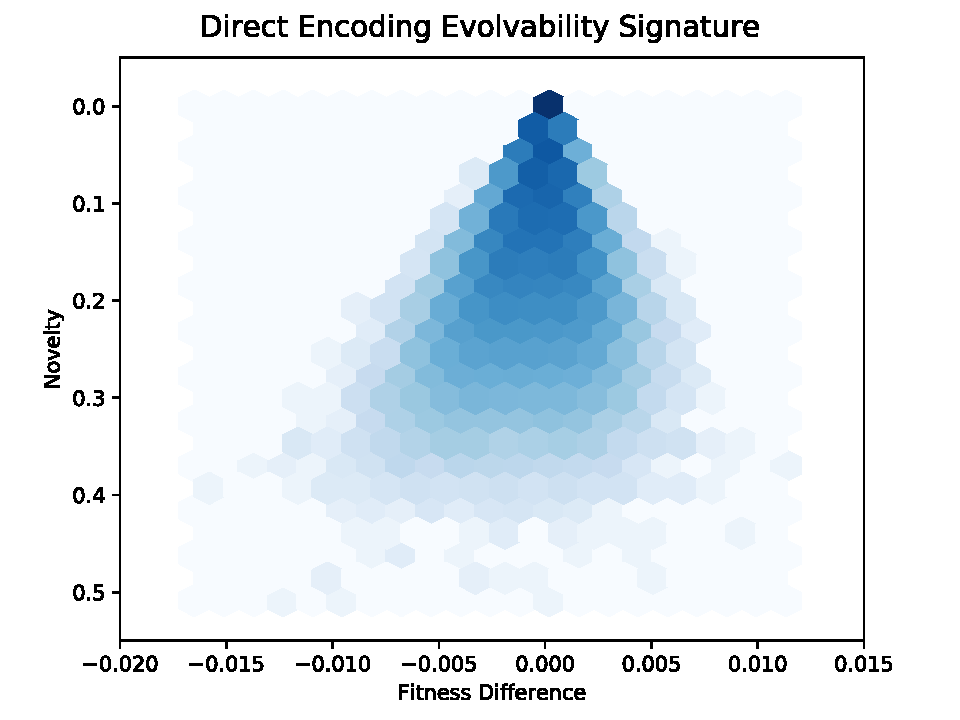
\includegraphics[width=\linewidth]{img/results/direct_es_unscaled}
    \subcaption{
      direct map
    }\label{fig:table_direct_es}
  \end{subfigure}
  \begin{subfigure}[b]{0.33\linewidth}
    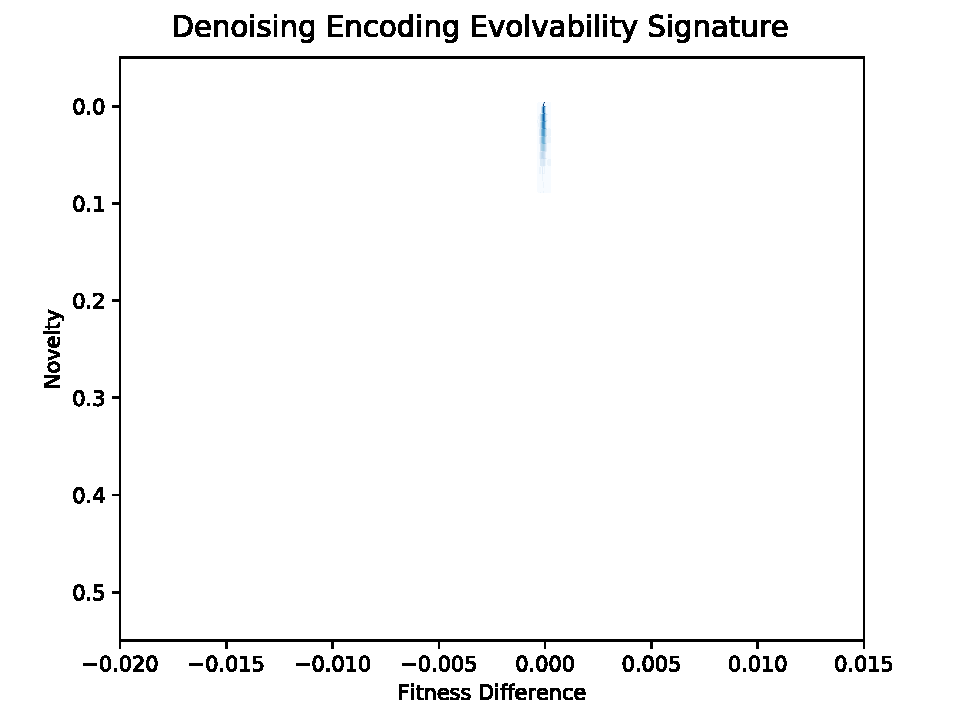
\includegraphics[width=\linewidth]{img/results/noise_es_unscaled}
    \subcaption{
      denoising map
    }\label{fig:table_noise_es}
  \end{subfigure}
  \begin{subfigure}[b]{0.33\linewidth}
    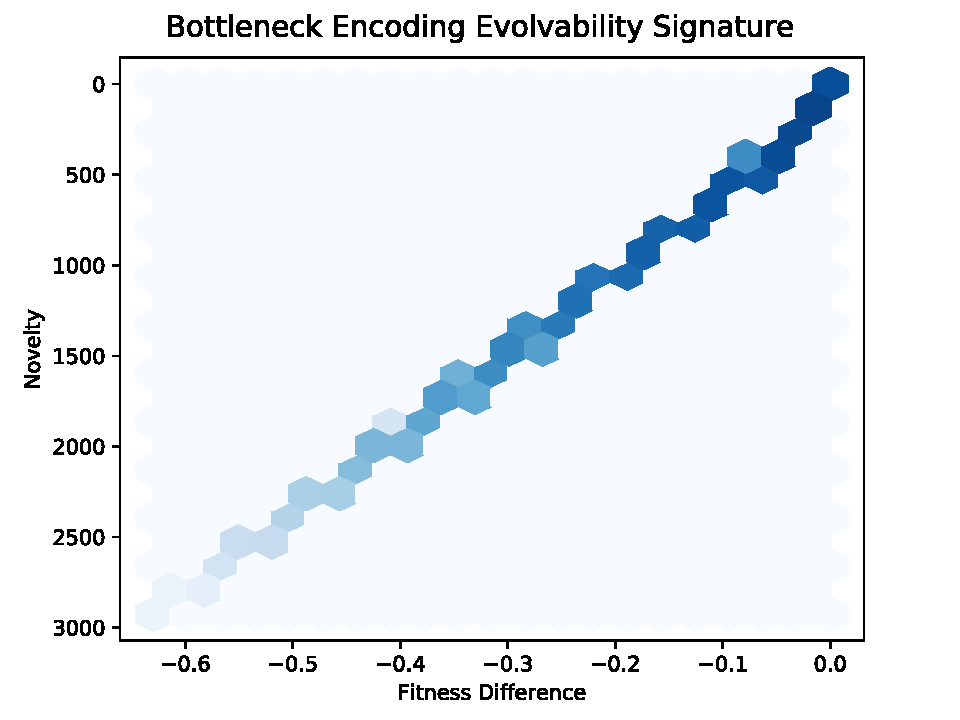
\includegraphics[width=\linewidth]{img/results/bottleneck_es_unscaled}
    \subcaption{
      bottleneck map
    }\label{fig:table_bottleneck_es}
  \end{subfigure}
  \caption{
    Evolvability signatures for three genotype-phenotype maps in the $n$-legged table problem domain.
    Note that subfigure \ref{fig:table_bottleneck_es} is presented with different axis scaling than subfigures \ref{fig:table_direct_es} and \ref{fig:table_noise_es}.
  }\label{fig:all_es}
\end{figure}


\end{frame}

\begin{frame}{TODO}

\begin{figure}
\foreach \n in {6,...,1}{%
\includegraphics[width=0.167\textwidth]{curly-guy/linear-\n}%
}%
\caption{TODO}
\end{figure}

\end{frame}

\begin{frame}{Result: Evolutionary Pacing}

\begin{figure}
  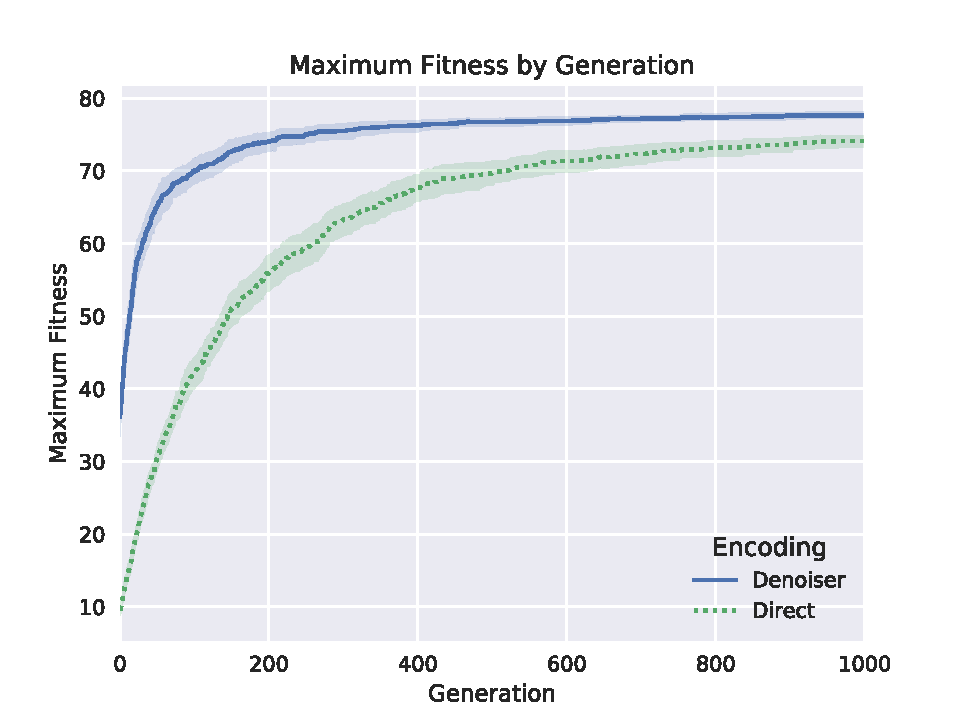
\includegraphics[width=0.8\linewidth]{img/results/scrabble_fit_vs_gen}
  \caption{
    Maximum individual fitness by generation in populations evolving in the Scrabble string domain.
    Bootstrapped 95\% confidence intervals are shaded along each curve.
  }\label{fig:scrabble_fit_vs_gen}
\end{figure}


\end{frame}


% \begin{frame}{Evolutionary Algorithm Parameters: Toy Problem}
%
% \begin{itemize}
% \item population size: 300
% \item tournament selection: $k = 5$
% \item crossover: two-point, two-parent, $p = 0.5$
% \item mutation: site-wise Gaussian perturbation
% \begin{itemize}
% \item training data, evolvability-signature experiments: $\mu = 0$, $\sigma = 0.1$, per-individual
% probability = 0.2, per-site probability = 0.01
% \item response-to-selection experiments: $\mu = 0$, $\sigma = 0.1$, per-individual probability = 0.2, per-site probability = 0.2 %TODO check this
% \footnote{for the bottleneck map, a per-site probability of 1 was employed}
% \end{itemize}
% \end{itemize}
%
% \end{frame}
%
% \begin{frame}{Denoising Autoencoder Hyperparameters: Toy Problem}
%
% \begin{itemize}
% \item 100-to-100 fully-connected linear layer without bias
% \item trained for 2500 epochs by stochastic gradient descent
% \item learning rate: $10^{−4}$
% \item momentum: 0.9
% \item batch size: 2048
% \item model parameters initialized uniformly between 0.005 and 0.015
% \item model parameters clamped in the range (0, 1
% \item during the training process, Gaussian
%   noise with $\mu = 0$, $\sigma = 0.025$ applied to input
% \item loss: mean square error of the difference between the original phenotype the reconstructed phenotype
% \end{itemize}
%
% \end{frame}
%
% \begin{frame}{Evolutionary Algorithm Parameters: Scrabble Problem}
%
% TODO
%
% \end{frame}
%
% \begin{frame}{Autoencoder Intuition: Bottlenecked}
%
% \begin{figure}
%   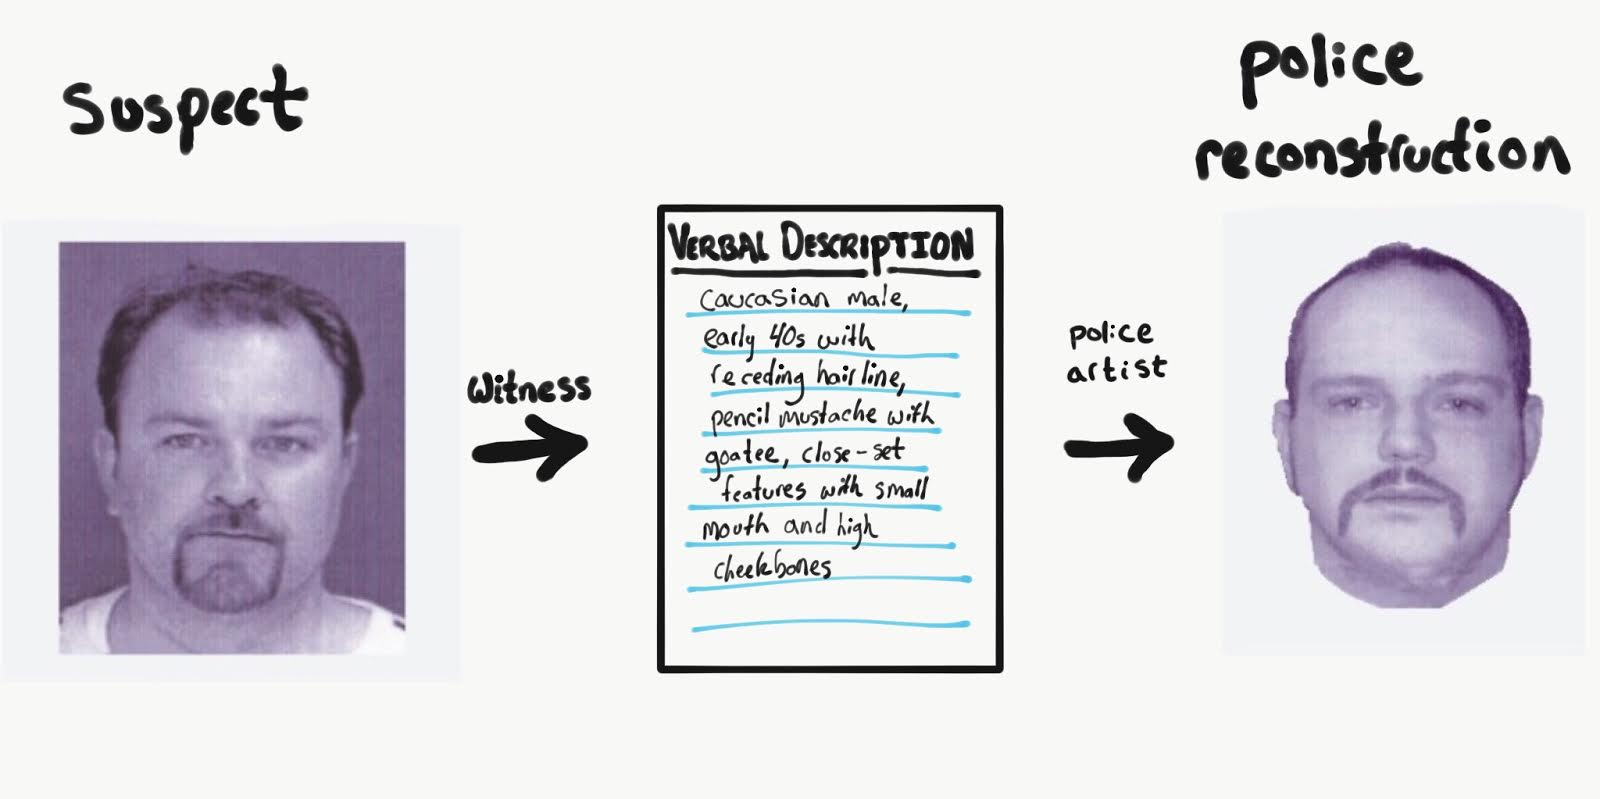
\includegraphics[width=\textwidth]{img/suspect}
%   \caption{
%   Schematic of hypothetical police composite process. Mug shot and composite reconstruction were taken from the Crime Scene Training Blog.
%   TODO cite
%   }
% \end{figure}
%
% \end{frame}
%
% \begin{frame}{Autoencoder Intuition: Denoiser}
%
% \begin{figure}
%   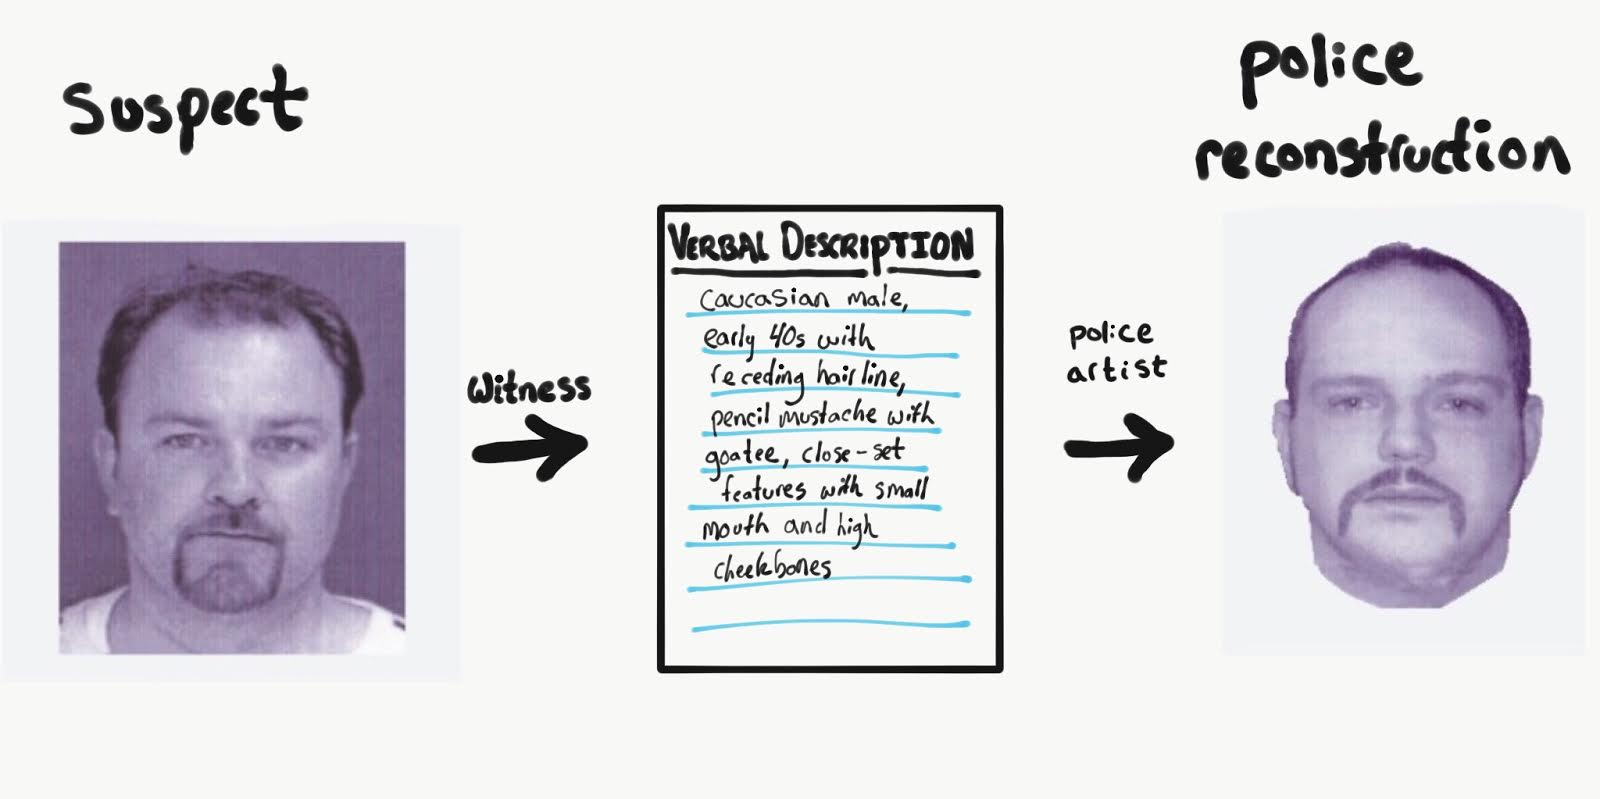
\includegraphics[width=\textwidth]{img/suspect}
%   \caption{
%   Schematic of hypothetical police composite process with suspect in disguise (incomplete input). Mug shot and composite reconstruction were taken from the Crime Scene Training Blog.
%   TODO cite
%   }
% \end{figure}
%
% \end{frame}

\begin{frame}{Autoencoder Intuition: Denoising}

\Large

\textbf{Why does this work?}

\pause

\begin{itemize}[<+->]
\item faces are a subset of all possible images
\item from arbitrary image, find nearest valid face
\item exploit symmetries, correlations, and universal characteristics of faces
\begin{itemize}[<+->]
\item ex. blue eyes correlated with blond hair (?)
\item ex. faces have same general eye-nose-mouth layout
\end{itemize}

\end{itemize}

\end{frame}


\begin{frame}{Autoencoder Intuition: Bottlenecked}

\Large

\textbf{Why does this work?}

\pause

\begin{itemize}[<+->]
\pause
\item faces are a subset of all possible images
\pause
\item don't need to specify which of all possible images, just need to specify which of all possible faces
\end{itemize}

\end{frame}


\begin{frame}{Intuition: Denoising G-P Map = Glorified Spell Checker}

\begin{figure}

\centering \Huge

\only<1>{

\dots\texttt{ns fed \fbox{o}xo sob }\dots

$\downarrow$

\texttt{\fbox{o}}

}

% \only<2>{
%
% \dots\texttt{la lob \fbox{\phantom{0}}re as s}\dots
%
% $\downarrow$
%
% \texttt{\fbox{o}}
%
% }

\only<2>{

\dots\texttt{lk y ag\fbox{x}r sned }\dots

$\downarrow$

\texttt{\fbox{a}}

}

\vspace{1ex}

\caption{
Example input-output pairs from trained Scrabble denoising autoencoder.
}

\end{figure}

\end{frame}

\begin{frame}{G-P Map Implementations: Toy}

\begin{columns}
\begin{column}{0.5\textwidth}
100-to-100 fully-connected layer
graphic: TODO
\begin{itemize}
\item intuition: averaging
\end{itemize}
\end{column}
\begin{column}{0.5\textwidth}
graphic: TODO
intuition: single underlying value
\end{column}
\end{columns}

\end{frame}
